\section{Реализация  сервиса для программной поддержки генерации расписания учебных заведений}

\subsection{Заполнение базы данных}

В идеальном сценарии для заполнения базы данных можно использовать API систем университета, хранящих такие данные как списки групп, преподавателей и учебные планы. Однако на момент написания данной выпускной квалификационной работы такая возможность отсутствует.

Альтернативный вариант – производить парсинг PDF файлов учебных планов и календарных учебных графиков, которые находятся в открытом доступе на сайте университета \cite{stankin:edu_programs} \cite{stankin:calendar}.

Однако существует третий вариант: переиспользовать написанный автором данной выпускной квалификационно работы в бакалавриате парсер \cite{github:grad_work_alpha} PDF файлов расписаний учебных занятий. Хоть это и не будет финальным решением, готовым для запуска системы в работу на пользу учебного заведения – это будет путём наименьшего сопротивления.

Этот подход также решит две другие проблемы, не имеющие элегантного решения. Тогда, как списки групп можно получить из соответствующего форума в ЭОС ФГБОУ ВО «МГТУ «СТАНКИН» \cite{stankin:groups}, актуальные списки преподавательского состава или таблицы со всеми учебными аудиториями и оборудованием найти не получится. В случае получения данных сразу из готового расписания за прошлый семестр можно определить и какие предметы ведут какие преподаватели, и какие предметы проводятся в каких аудиториях.

\subsubsection{Процесс популяции базы данных}

Скачать все расписания на текущий семестр можно в соответствующем форуме в ЭОС ФГБОУ ВО «МГТУ «СТАНКИН» \cite{stankin:schedule}.

Для заполнения базы данных требуемыми данными была написана специальная вспомогательная программа \cite{github:subject_parser}, производящая парсинг данных и приводящая их в нужную структуру и формат в SQLite (см. Рис.~\ref{fig:db}).

\begin{figure}[H]
	\centering
	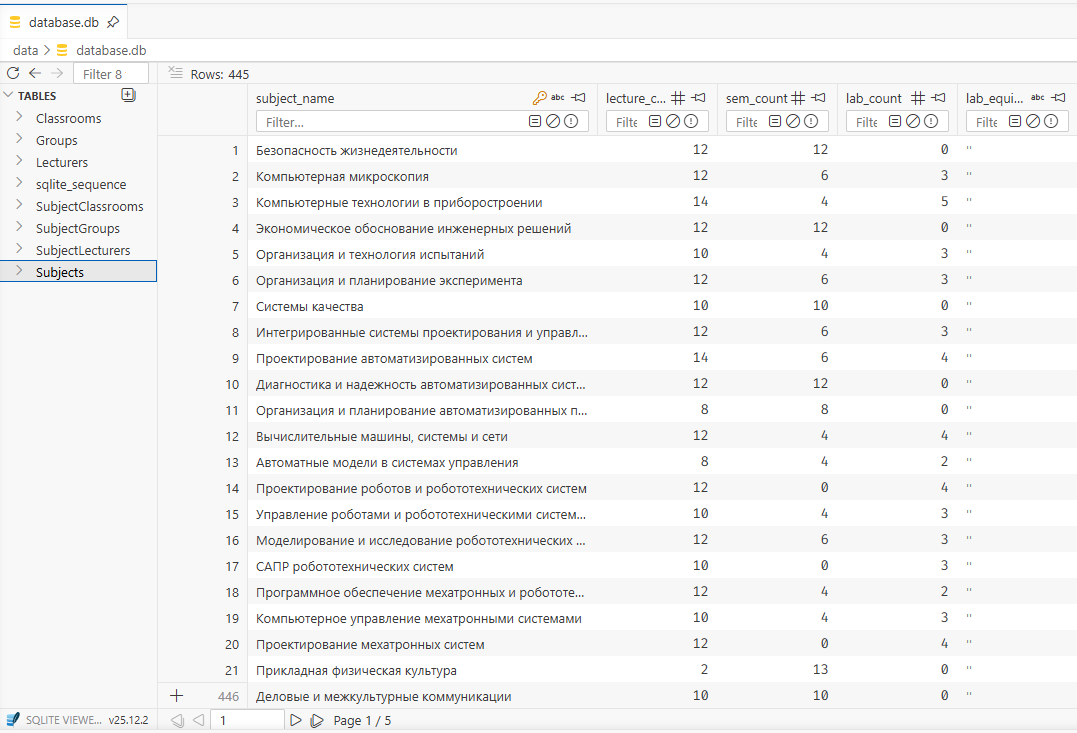
\includegraphics[width=1\textwidth]{images/ch5/db.png}
	\caption{Заполненная БД}
	\label{fig:db}
\end{figure}

\subsection{Сервер}

Как уже описывалось в предыдущей главе, в качестве основы вычислительной части проекта был выбран Polars. На основе его декларативного языка программирования был реализован алгоритм решения задачи.
Все основные методы были обёрнуты в REST API благодаря FastAPI, а Swagger позволил упростить процесс написания будущего клиента.

Также были разработаны дополнительные инструменты визуализации расписания для упрощения дебага текущего состояния расписания, как например интерактивная визуализация всего расписания на семестр (см. Рис.~\ref{fig:debug}).

\begin{figure}[H]
	\centering
	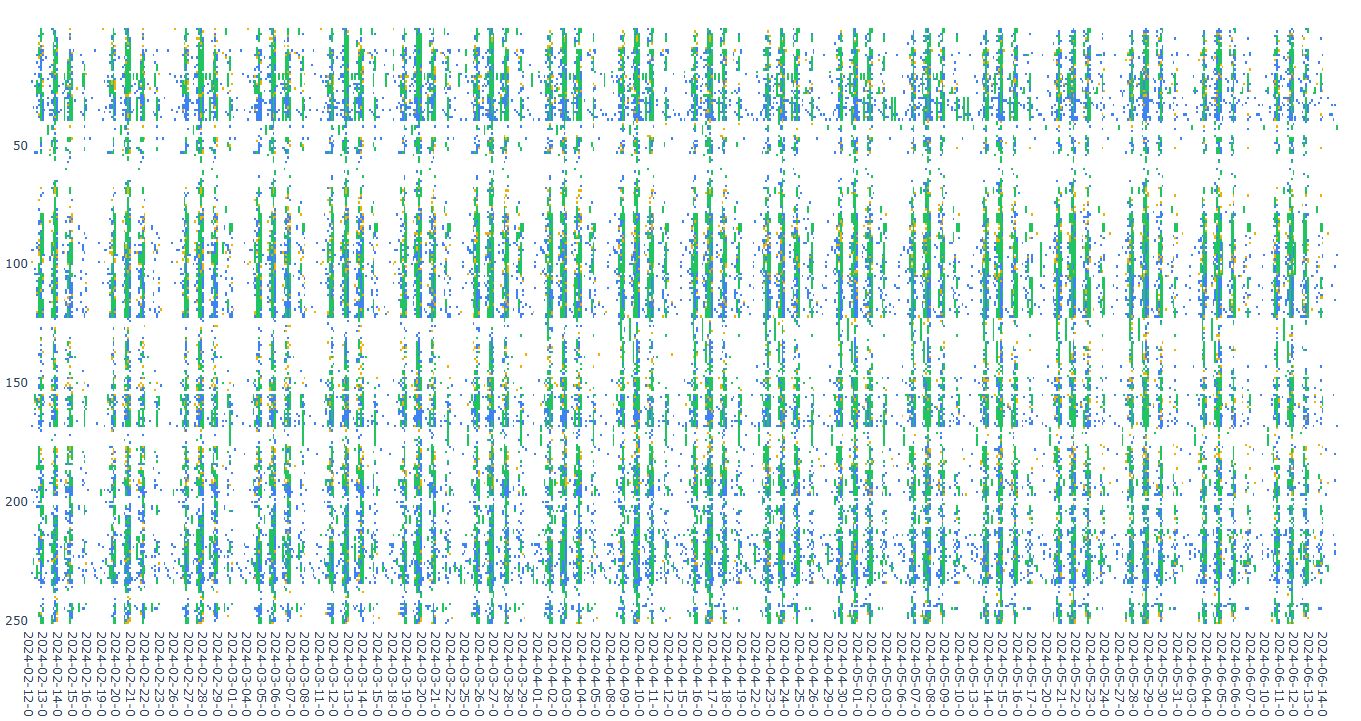
\includegraphics[width=1\textwidth]{images/ch5/debug.png}
	\caption{Интерактивная визуализация расписания университета на семестр}
	\label{fig:debug}
\end{figure}

\subsection{Клиент}

В роли клиента было написано веб-приложение на базе Nuxt 4 и Vue 3.5 (см. Рис.~\ref{fig:client}), а технология progressive web application (PWA) позволяет установить сайт как нативное приложения на любое современное устройство, поддерживающие браузер. То есть генерацию расписания можно производить даже с некоторых холодильников или наручных часов.

\begin{figure}[H]
	\centering
	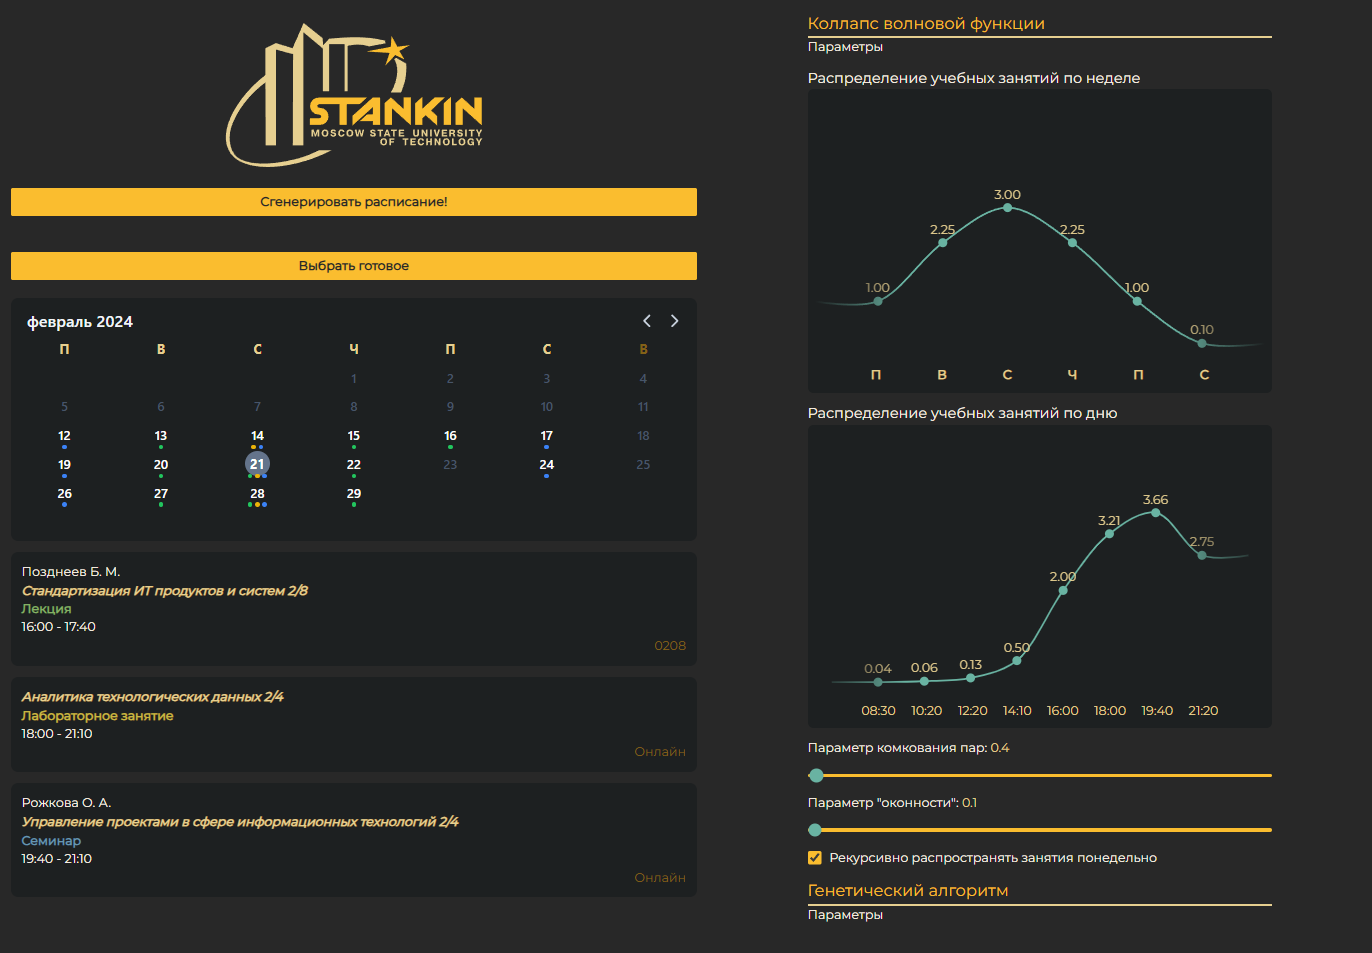
\includegraphics[width=1\textwidth]{images/ch5/client.png}
	\caption{Клиент}
	\label{fig:client}
\end{figure}

\subsection{Вывод по пятой главе}

Была реализована программная основа сервиса для генерации расписания учебных занятий. Для системы была реализована трёхзвенная архитектура, обеспечивающая разделение ответственности между хранилищем данных, серверной логикой и пользовательским интерфейсом. Был подготовлен механизм заполнения БД на основе доступных источников данных.

На стороне сервера реализована бизнес-логика и REST API для взаимодействия с клиентской частью и внешними компонентами системы. На стороне клиента разработано веб-приложение, позволяющее удобно работать с сервисом через браузер. В результате получена работоспособная система, пригодная для дальнейшего развития и последующей интеграции в более полный процесс автоматизированного формирования расписания.
